\documentclass[12pt]{article}%
\usepackage{amsfonts}
\usepackage{fancyhdr}
\usepackage{comment}
\usepackage[a4paper, top=2.5cm, bottom=2.5cm, left=2.2cm, right=2.2cm]%
{geometry}
\usepackage{times}
\usepackage{amsmath}
\usepackage{changepage}
\usepackage{amssymb}
\usepackage{enumitem}


\usepackage{graphicx}
\graphicspath{ {./images/} }


\usepackage{algorithm}% http://ctan.org/pkg/algorithm
\usepackage{algpseudocode}% http://ctan.org/pkg/algorithmicx


\usepackage{scrextend}

\usepackage{graphicx}%
\setcounter{MaxMatrixCols}{30}
\newtheorem{theorem}{Theorem}
\newtheorem{acknowledgement}[theorem]{Acknowledgement}

\newtheorem{axiom}{Axiom}
\newtheorem{case}[theorem]{Case}
\newtheorem{claim}[theorem]{Claim}
\newtheorem{conclusion}[theorem]{Conclusion}
\newtheorem{condition}[theorem]{Condition}
\newtheorem{conjecture}[theorem]{Conjecture}
\newtheorem{corollary}[theorem]{Corollary}
\newtheorem{criterion}[theorem]{Criterion}
\newtheorem{definition}[theorem]{Definition}
\newtheorem{example}[theorem]{Example}
\newtheorem{exercise}[theorem]{Exercise}
\newtheorem{lemma}[theorem]{Lemma}
\newtheorem{notation}[theorem]{Notation}
\newtheorem{problem}[theorem]{Problem}
\newtheorem{proposition}[theorem]{Proposition}
\newtheorem{remark}[theorem]{Remark}
\newtheorem{solution}[theorem]{Solution}
\newtheorem{summary}[theorem]{Summary}
\newenvironment{proof}[1][Proof]{\textbf{#1.} }{\ \rule{0.5em}{0.5em}}

\newcommand{\Q}{\mathbb{Q}}
\newcommand{\R}{\mathbb{R}}
\newcommand{\C}{\mathbb{C}}
\newcommand{\Z}{\mathbb{Z}}


\documentclass{minimal}
\usepackage{mathtools}
\DeclarePairedDelimiter\ceil{\lceil}{\rceil}
\DeclarePairedDelimiter\floor{\lfloor}{\rfloor}
\begin{document}

\title{Homework 5}
\author{Jeffery Russell}
\date{\today}
\maketitle

\section{BFS}

\begin{enumerate}[label=(\alph*)]
    \item CLRS 22.2-2\\
    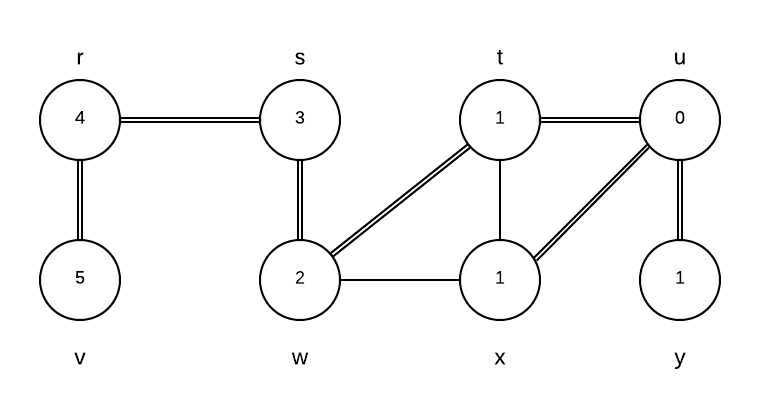
\includegraphics[width=\textwidth]{bfs}

\begin{table}[h]
\begin{tabular}{l|l|l|l|l|l|l|l|l}
Vertex              & u   & t & s & r & v & w & x & y \\ \hline
$\pi$ & Nil & u & w & s & r & t & u & u \\ \hline
d                   & 0   & 1 & 3 & 4 & 5 & 2 & 1 & 1
\end{tabular}
\end{table}
    
    \item Show that using a single bit to store each vertex color suffices by arguing that the BFS procedure would produce the same result if line 18 were removed.\\
    
    In the BFS algorithm provided to us, they keep track of the vertex as being white when not-visited,
    gray when they are visiting their neighbors and black when finished visiting all of the neighbors have been added to the queue. However, the algorithm never actually uses the fact that the color of the vertex has changed to black so it is sufficient to exclude line 18 where the color is set to black. Since this BFS algorithm is only interested if the vertex has been visited yet or not, a single bit would suffice, 0 to represent white and 1 to represent gray. 
    
    
    \item CLRS 22.2-5\\
    
    The value assigned to d will not change no-matter what order the vertices appear in each adjacency list. However, changing the order of vertices could change the value of the predecessors. Take figure 22.3 for example, to get to vertex w we could have taken either the edge from t or from x. I decided to traverse the adjacent vertices in alphabetical order so I went from t to w and w got a distance of 2 and it's predecessor was set to t. However, if I went from x to x the distance would still be 2, but, it's predecessor would be set to x instead. This property is inherit in the BFS algorithm because it looks for shortest path and does not make any assumptions about the ordering of the adjacency lists.
    
\end{enumerate}

\section{Matrix-Chain Multiplication}
Consider the following chain of six matrices: $A_1$, $A_2$, $A_3$,
$A_4$, $A_5$, and $A_6$, where $A_1$ is $5\times 10$, $A_2$ is
$10\times 3$, $A_3$ is $3\times 12$, $A_4$ is $12\times 5$, $A_5$ is
$5\times 50$, and $A_6$ is $50\times 6$.  Find an optimal
parenthesization of this matrix-chain.  Show both the table containing
the optimal number of scalar operations for all slices and the choice
table.

Answer with 2010 scalar multiplications:\\
((A_1A_2)((A_3A_4)(A_5A_6)))

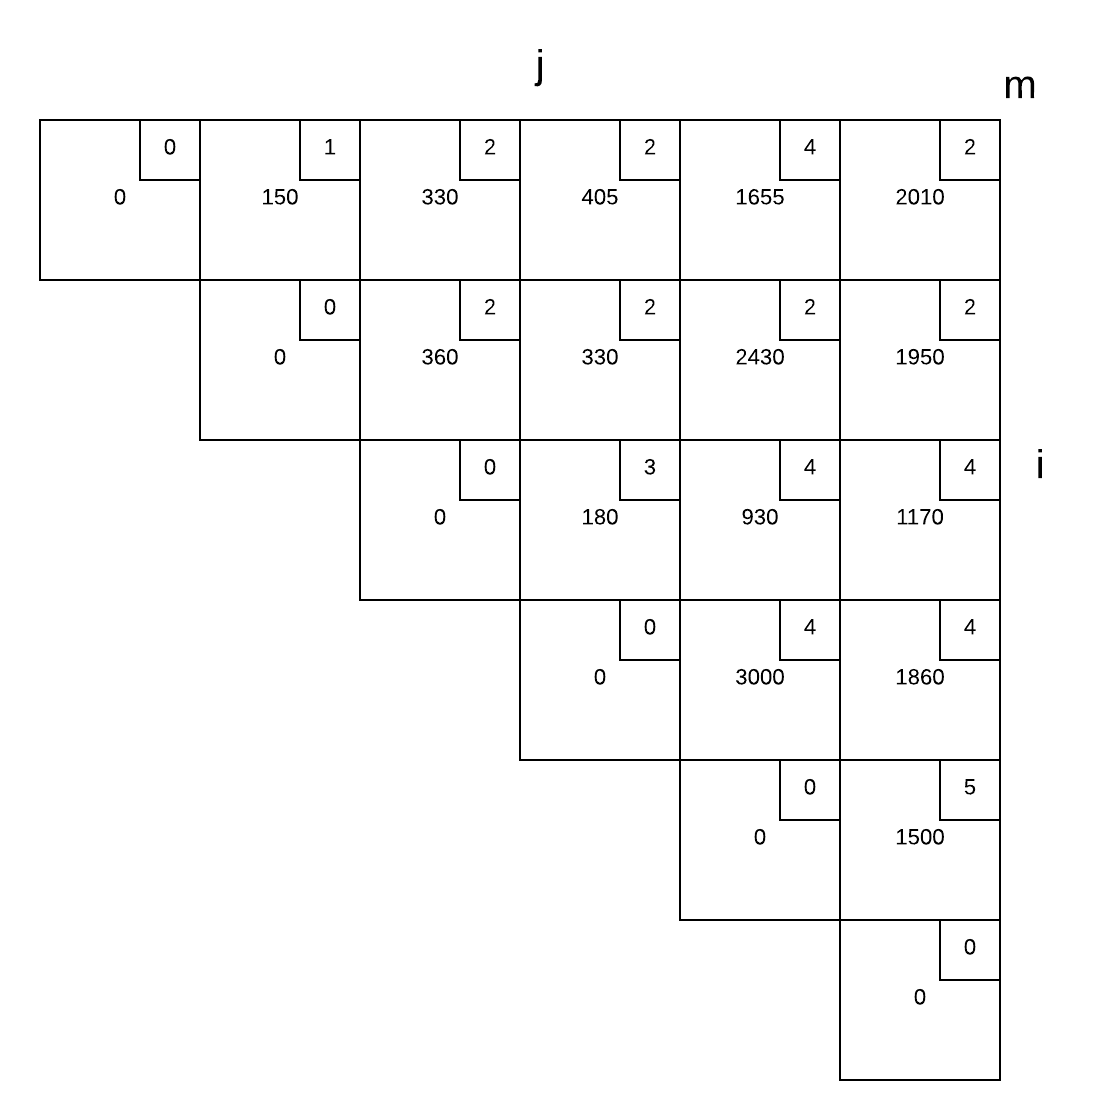
\includegraphics[]{images/matrixMult.png}





\section{Matrix-Chain Multiplication Parenthesize}
\begin{enumerate}[label=(\alph*)]
    \item CLRS 15.3-1\\
    Which is a more efficient way to determine the optimal number of multiplications
in a matrix-chain multiplication problem: enumerating all the ways of parenthesizing the product and computing the number of multiplications for each, or running
RECURSIVE-MATRIX-CHAIN ? Justify your answer.

\textbf{Answer}\\
Running the RECURSIVE-MATRIX-CHAIN is more efficient. My argument for this claim is that asymptotically RECURSIVE-MATRIX-CHAIN is faster than enumerating all the solutions.\\

\textbf{Enumeration:}\\
As stated in CLS section 15.2, the running time of enumeration is $\Omega(\frac{4^n}{n^\frac{3}{2}})$

\textbf{RECURSIVE-MATRIX-CHAIN:}\\
In section 15-3 of the text book it proved that the RECURSIVE-MATRIX-CHAIN ran in $\Omega(2^n)$. This is better than the lower bound for Enumeration; however, comparing two lower bounds of functions will not help us prove that one actually runs better than the other. To find an upper bound we will reverse the inequality used to find the lower bound.

$
T(n) \leq 2 \sum_{i=1}^{n -1} T(i) + n
$

Instead of solving this recurrence with iteration, I will prove that it has an upper bound of $O(3.5^n)$ using induction.

\textbf{Lemma 1:} For any $n \in N, $T(n) \leq  2\sum_{i=1}^{n -1} T(i) + n \leq 3.5^n$\\
\textbf{Proof via Induction:}\\
\textbf{BaseCase:} n=1
\begin{addmargin}[6em]{2em}% 1em left, 2em right
    $LHS = 2\sum^{1-1}_{1}T(i) + 1$\\
    $= 1$\\
    $RHS = 3.5^1$\\
    $= 3.5$\\
    $LHS \leq RHS$\\
    $\Box$\\
\end{addmargin}\\

\textbf{Inductive Step:}\\
Assume proposition is true for all n, show that n+1 follows.\\
\begin{addmargin}[6em]{2em}% 1em left, 2em right
$LHS = T(n + 1) =  2\sum_{i=1}^{n + 1 -1} T(i) + n + 1$\\
$= 2(1.4(3.5)^n - 1.4) + n +  1$\textsl{By I.H}\\
$= 2.8(3.5)^n - 1.8 + n$\\
$RHS = 3.5^{n+ 1}$\\
$LHS \leq RHS$ \textsl{For sufficiently large n}\\
$\Box$\\
\end{addmargin}

\textbf{Corollary 1:}
By lemma 1; T(n) is $O(3.5^n)$\\

Since enumerations runs in $\Omega(\frac{4^n}{n^\frac{3}{2}})$ and the recursive solution runs in 
$O(3.5^n)$, the RECURSIVE-MATRIX-CHAIN is asomtotically faster. 
    \item Consider a variant of the matrix-chain multiplication problem in which the goal is to parenthesize the sequence of matrices so as to maximize the number of scalar multiplications. Does this problem exhibit optimal substructure?\\
    
\textbf{Answer}\\
Yes. If we can work to minimize the number of scalar multiplications, we can similarly work to maximize the number of scalar multiplications. A lot like when we worked to use dynamic programming to to minimize the number of multiplications, we can modify our champion algorithm to instead select the k associated with the maximum amount of scalar multiplications.

\end{enumerate}

\section{Text Formatting}

Consider the problem of neatly printing a paragraph on the
  screen (or on a printer).  The input text is a sequence $S$ of $n$
  words (represented as strings) of lengths $\ell_1, \ldots, \ell_n $
  (measured in characters). The input bound $M$ is the maximum number
  of characters a line can hold.  The key to neatly printing a
  paragraph is to identify in the text sequence the lines of the
  paragraph so that new-lines can be placed at the end of each line.
  We can formalize the notion of the ``badness'' of a line as the
  number of extra space characters at the end of the line or $\infty$
  if the bound $M$ is exceeded.  We can formalize the notion of the
  ``badness'' of a paragraph as the badness of the worst (i.e.,
  maximum) line of the paragraph not including the last line.  Thus to
  identify the lines for a neat paragraph, we seek to minimize the
  badness of the paragraph.

\begin{enumerate}[label=(\alph*)]
    \item If a given line contains words $i$ through $j$, and we leave
  exactly one space between words, the number of extra space
  characters at the end of the line is $M - j + i - \sum_{k=i}^{j}
  \ell_k$.  Write a mathematical function $es(S, M, i, j)$ that
  computes the number of extra space characters at the end of a line.
  
$$  
es(S,M, i,j) = 
  \begin{cases}
   M- |S[i]| & \text{if } i=j \\
    es(S, M-|S[i]| -1, i + 1, j)      & \text{otherwise}
  \end{cases}
$$

    
    \item (Project)\\
    
    \item Use the function es to write a mathematical function bl(S, M, i, j) that computes line badness.\\

$$
bl(S,M, i,j) = 
  \begin{cases}
   \infty & \text{if } es(S,M,i,j) < 0 \\
    es(S,M,i,j)     & \text{otherwise}
  \end{cases}
$$
    
    \item (Project)\\
    
    \item  Write a recursive mathematical function mb(S, M) that computes the minimum paragraph badness (using
slicing).\\

$$
mb(S,M) = 
  \begin{cases}
   0 & \text{if } bl(S, M, 1, |S|)  \neq  \infty \\
   min\{max\{bl(S, M, 1, k), mb(S[k+1:], M)\} |\\
    1 \leq k \leq |S| -1\}    & \text{otherwise}
  \end{cases}
$$

\item Write a recursive mathematical function mb'
(S, M, i) where mb'
(S, M, i) = mb(S[i :], M).\\


$$
mb(S, M, i) = 
  \begin{cases}
   0 & \text{if } bl(S, M, i, |S|)  \neq  \infty \\
   min\{max\{bl(S, M, i, k), mb'(S, M, k)\} |\\
    i + 1 \leq k \leq |S| -1\}    & \text{otherwise}
  \end{cases}
$$

\item (Project) \\
\item (Project) \\
\item (Project) \\

    
\end{enumerate}


\section{Bellman-Ford Algorithm}
CLRS 24.1-1\\
Run the Bellman-Ford algorithm on the directed graph of Figure 24.4, using vertex z as the source. In each pass, relax edges in the same order as in the figure, and
show the d and $\pi$ values after each pass. Now, change the weight of edge (z,x)
to 4 and run the algorithm again, using s as the source.

% First Pass
% 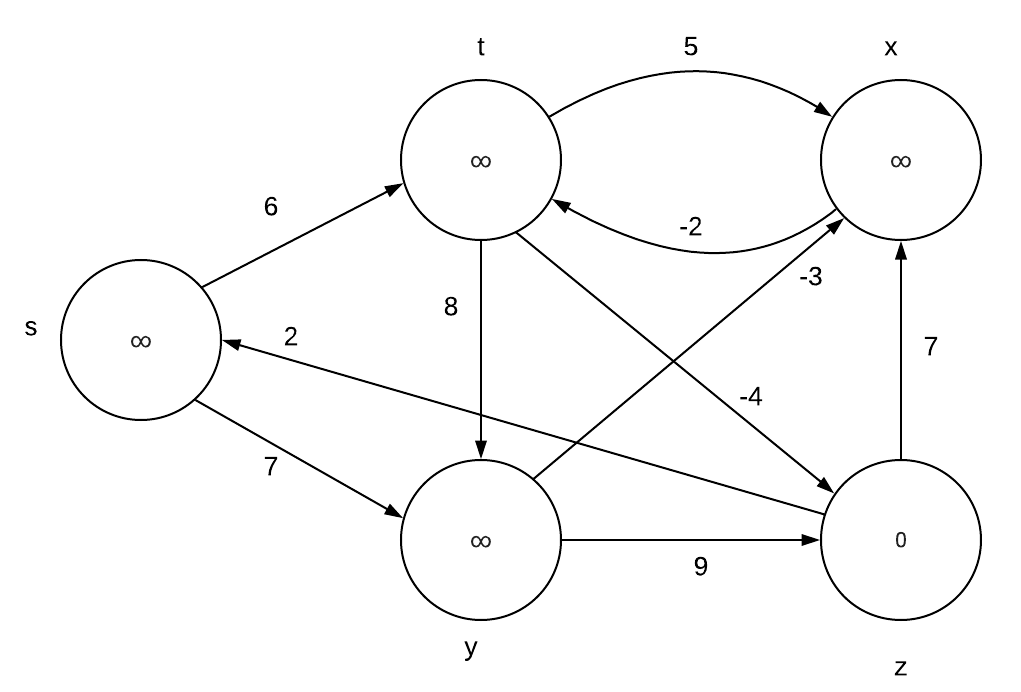
\includegraphics[width=\textwidth]{Ford1}

% Second Pass
% 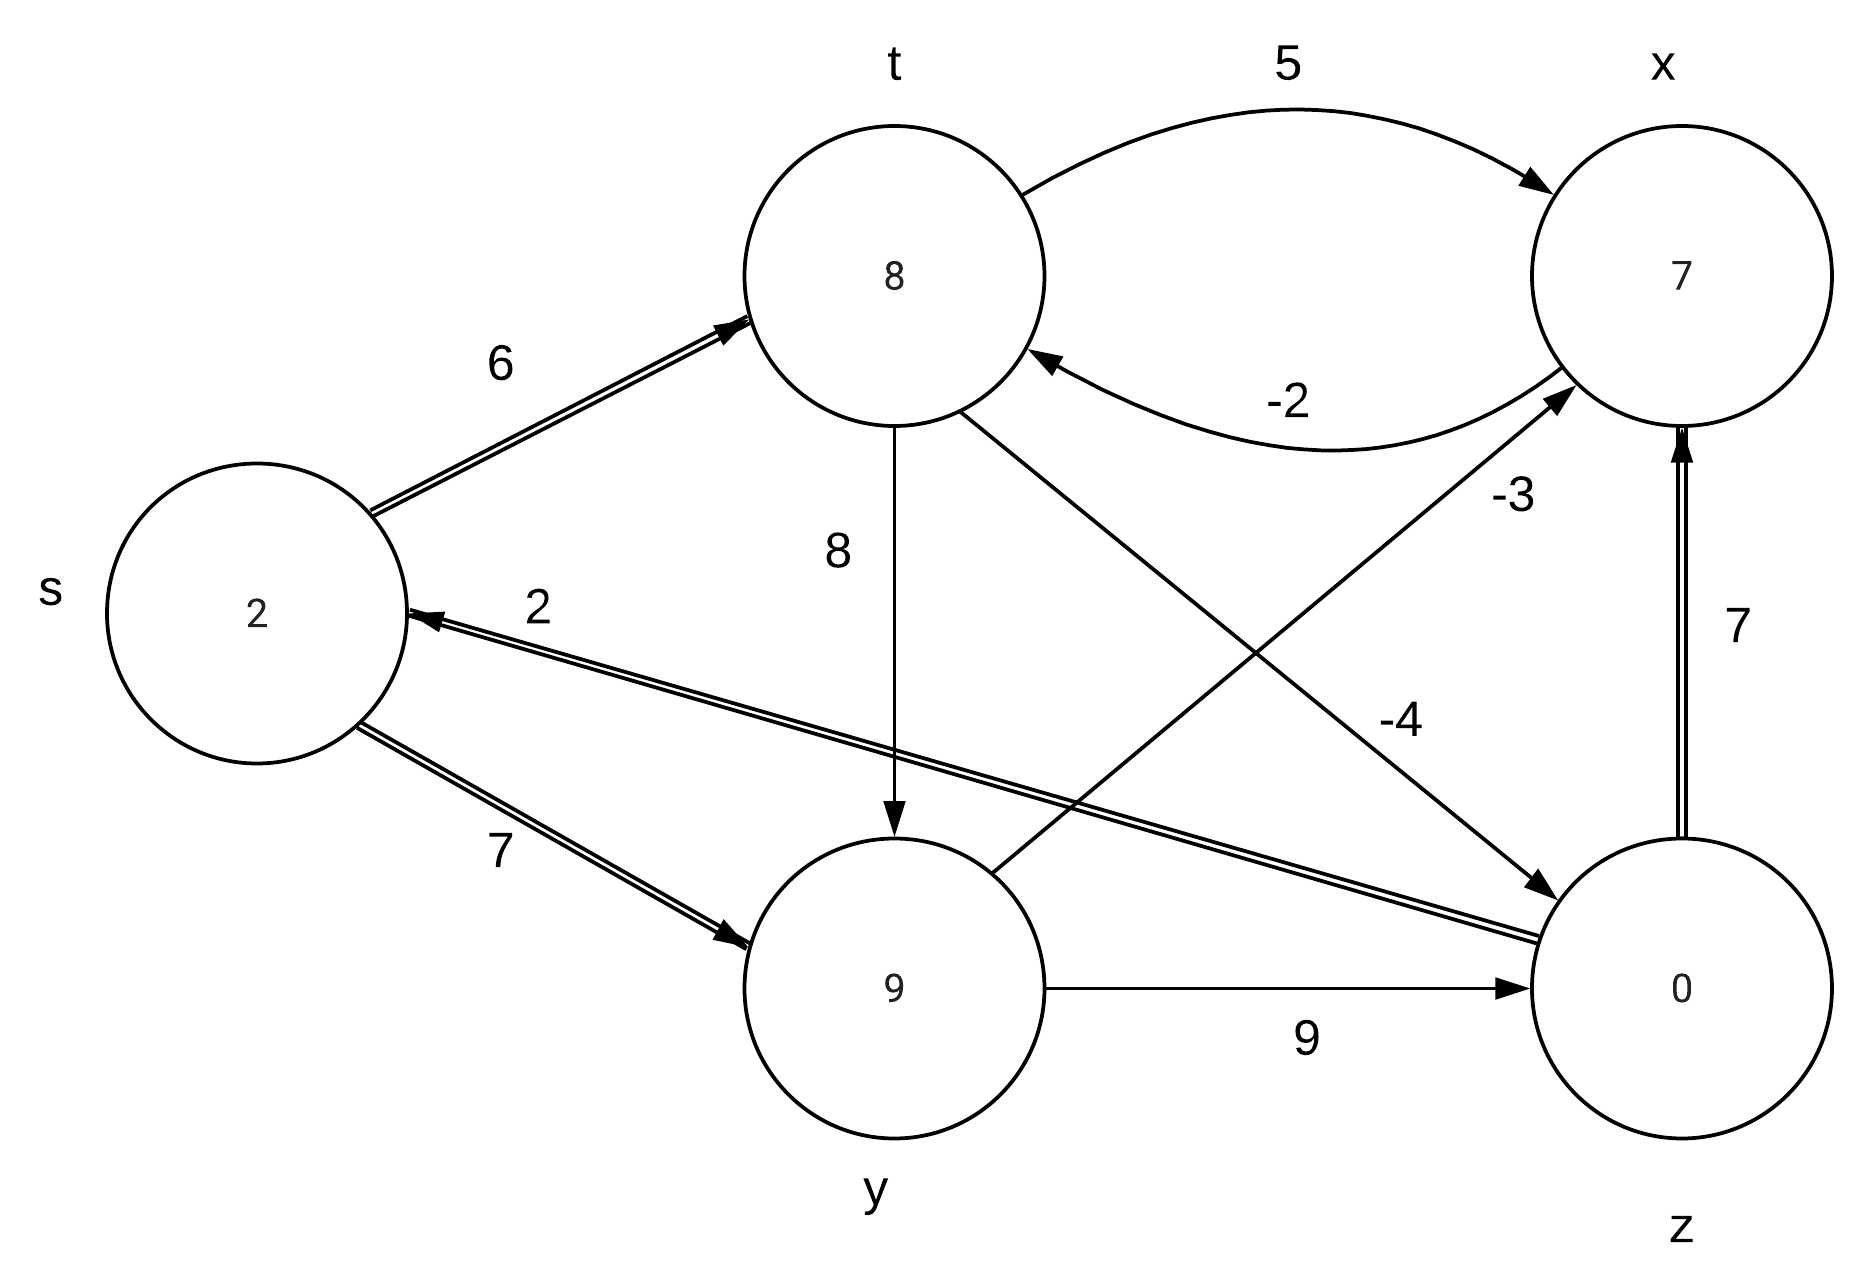
\includegraphics[]{Ford2}

% Final Pass
% 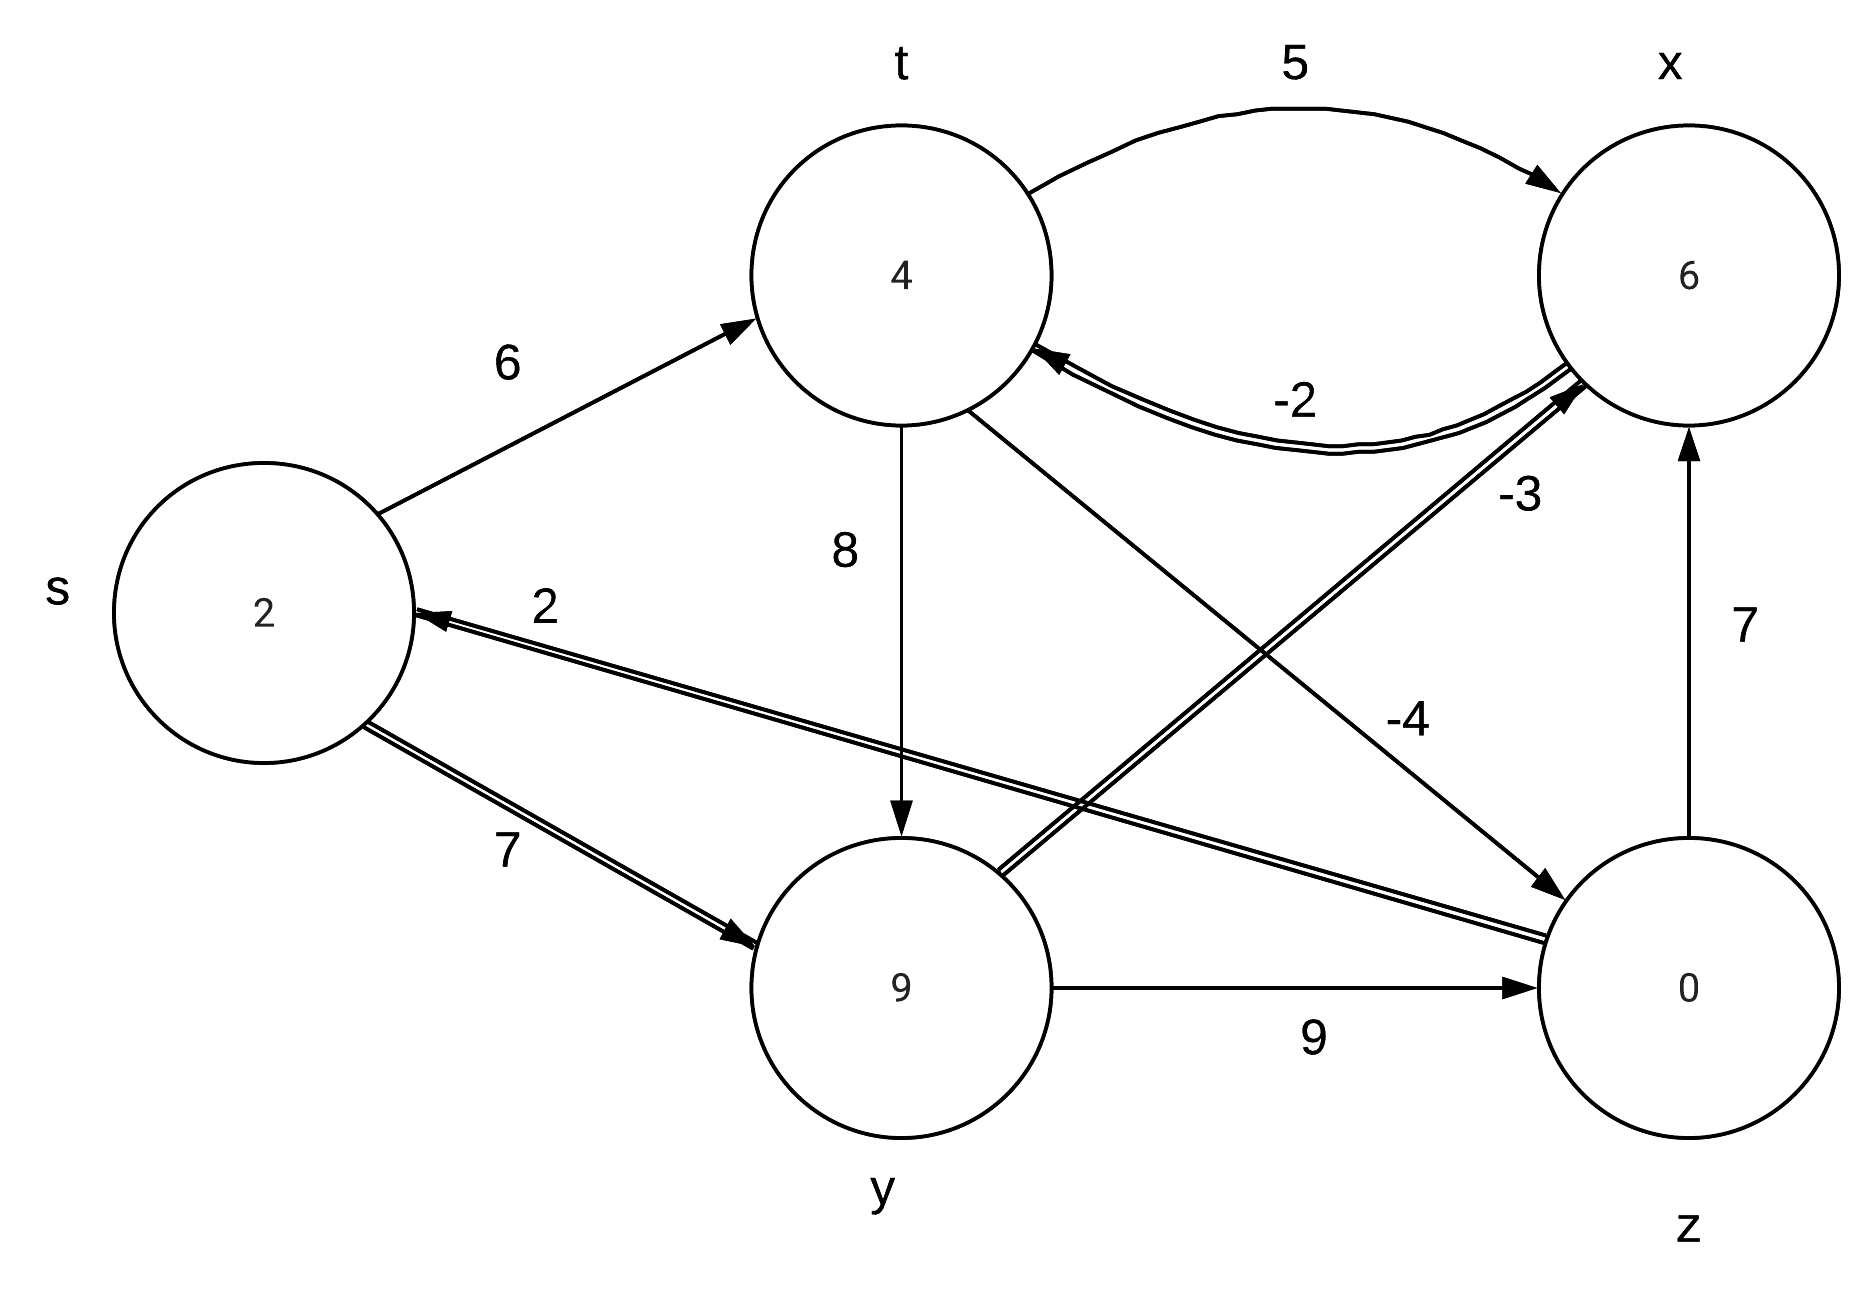
\includegraphics[]{Ford3}

Part a:
\begin{center}
  \makebox[\textwidth]{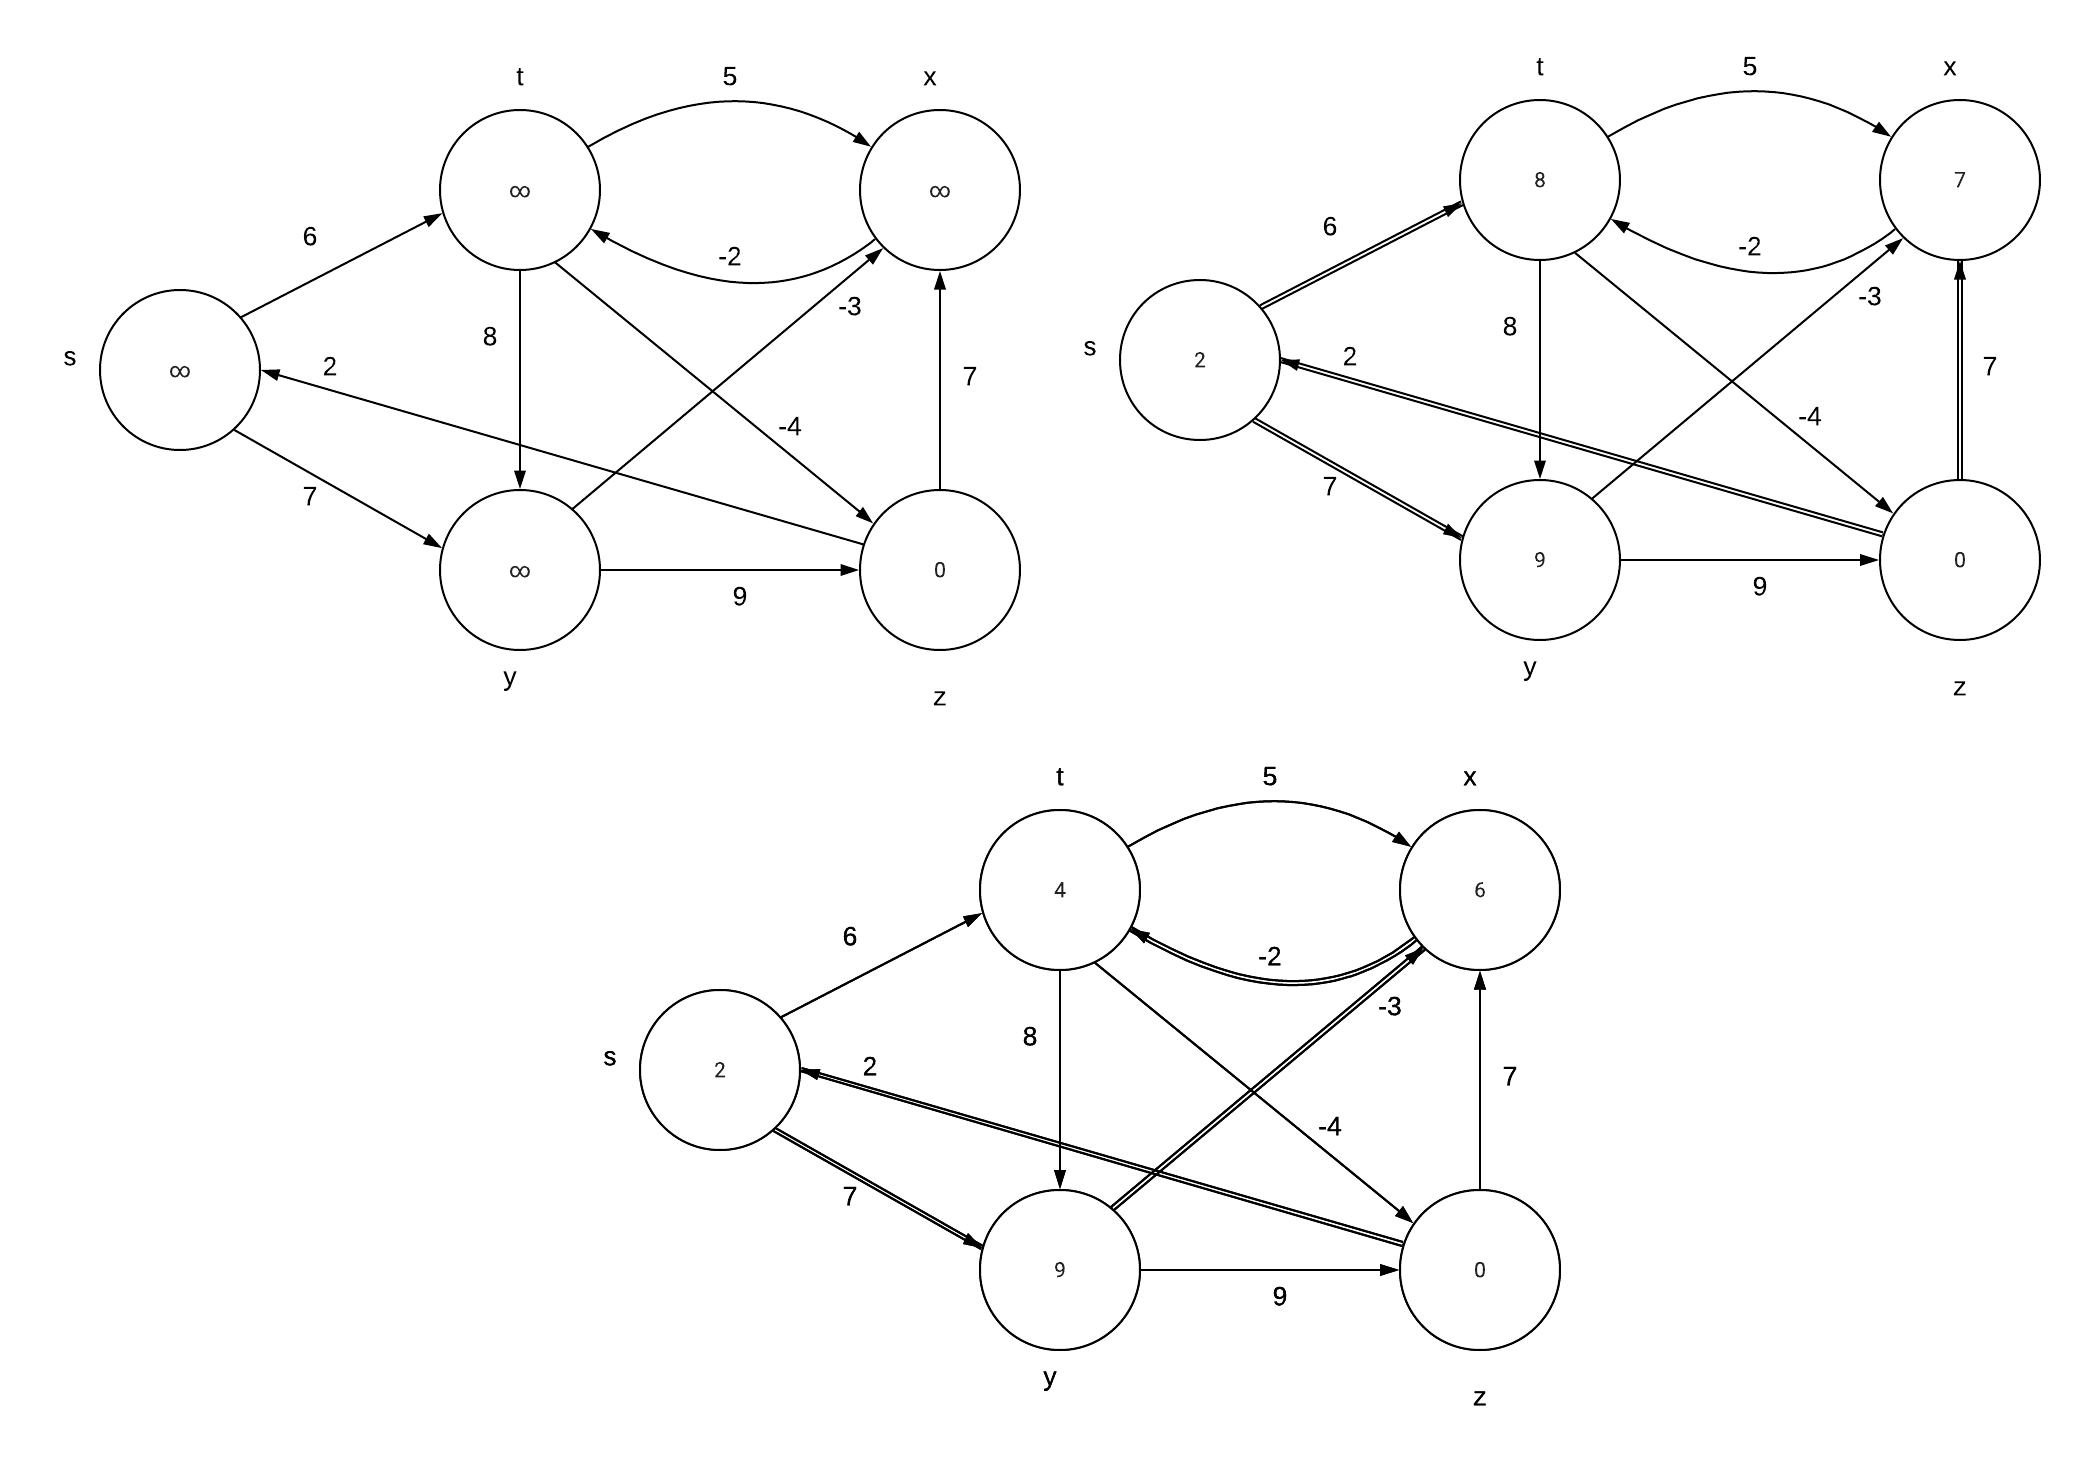
\includegraphics[width=\paperwidth]{images/afinal.png}}
\end{center}

Part b:
\begin{center}
  \makebox[\textwidth]{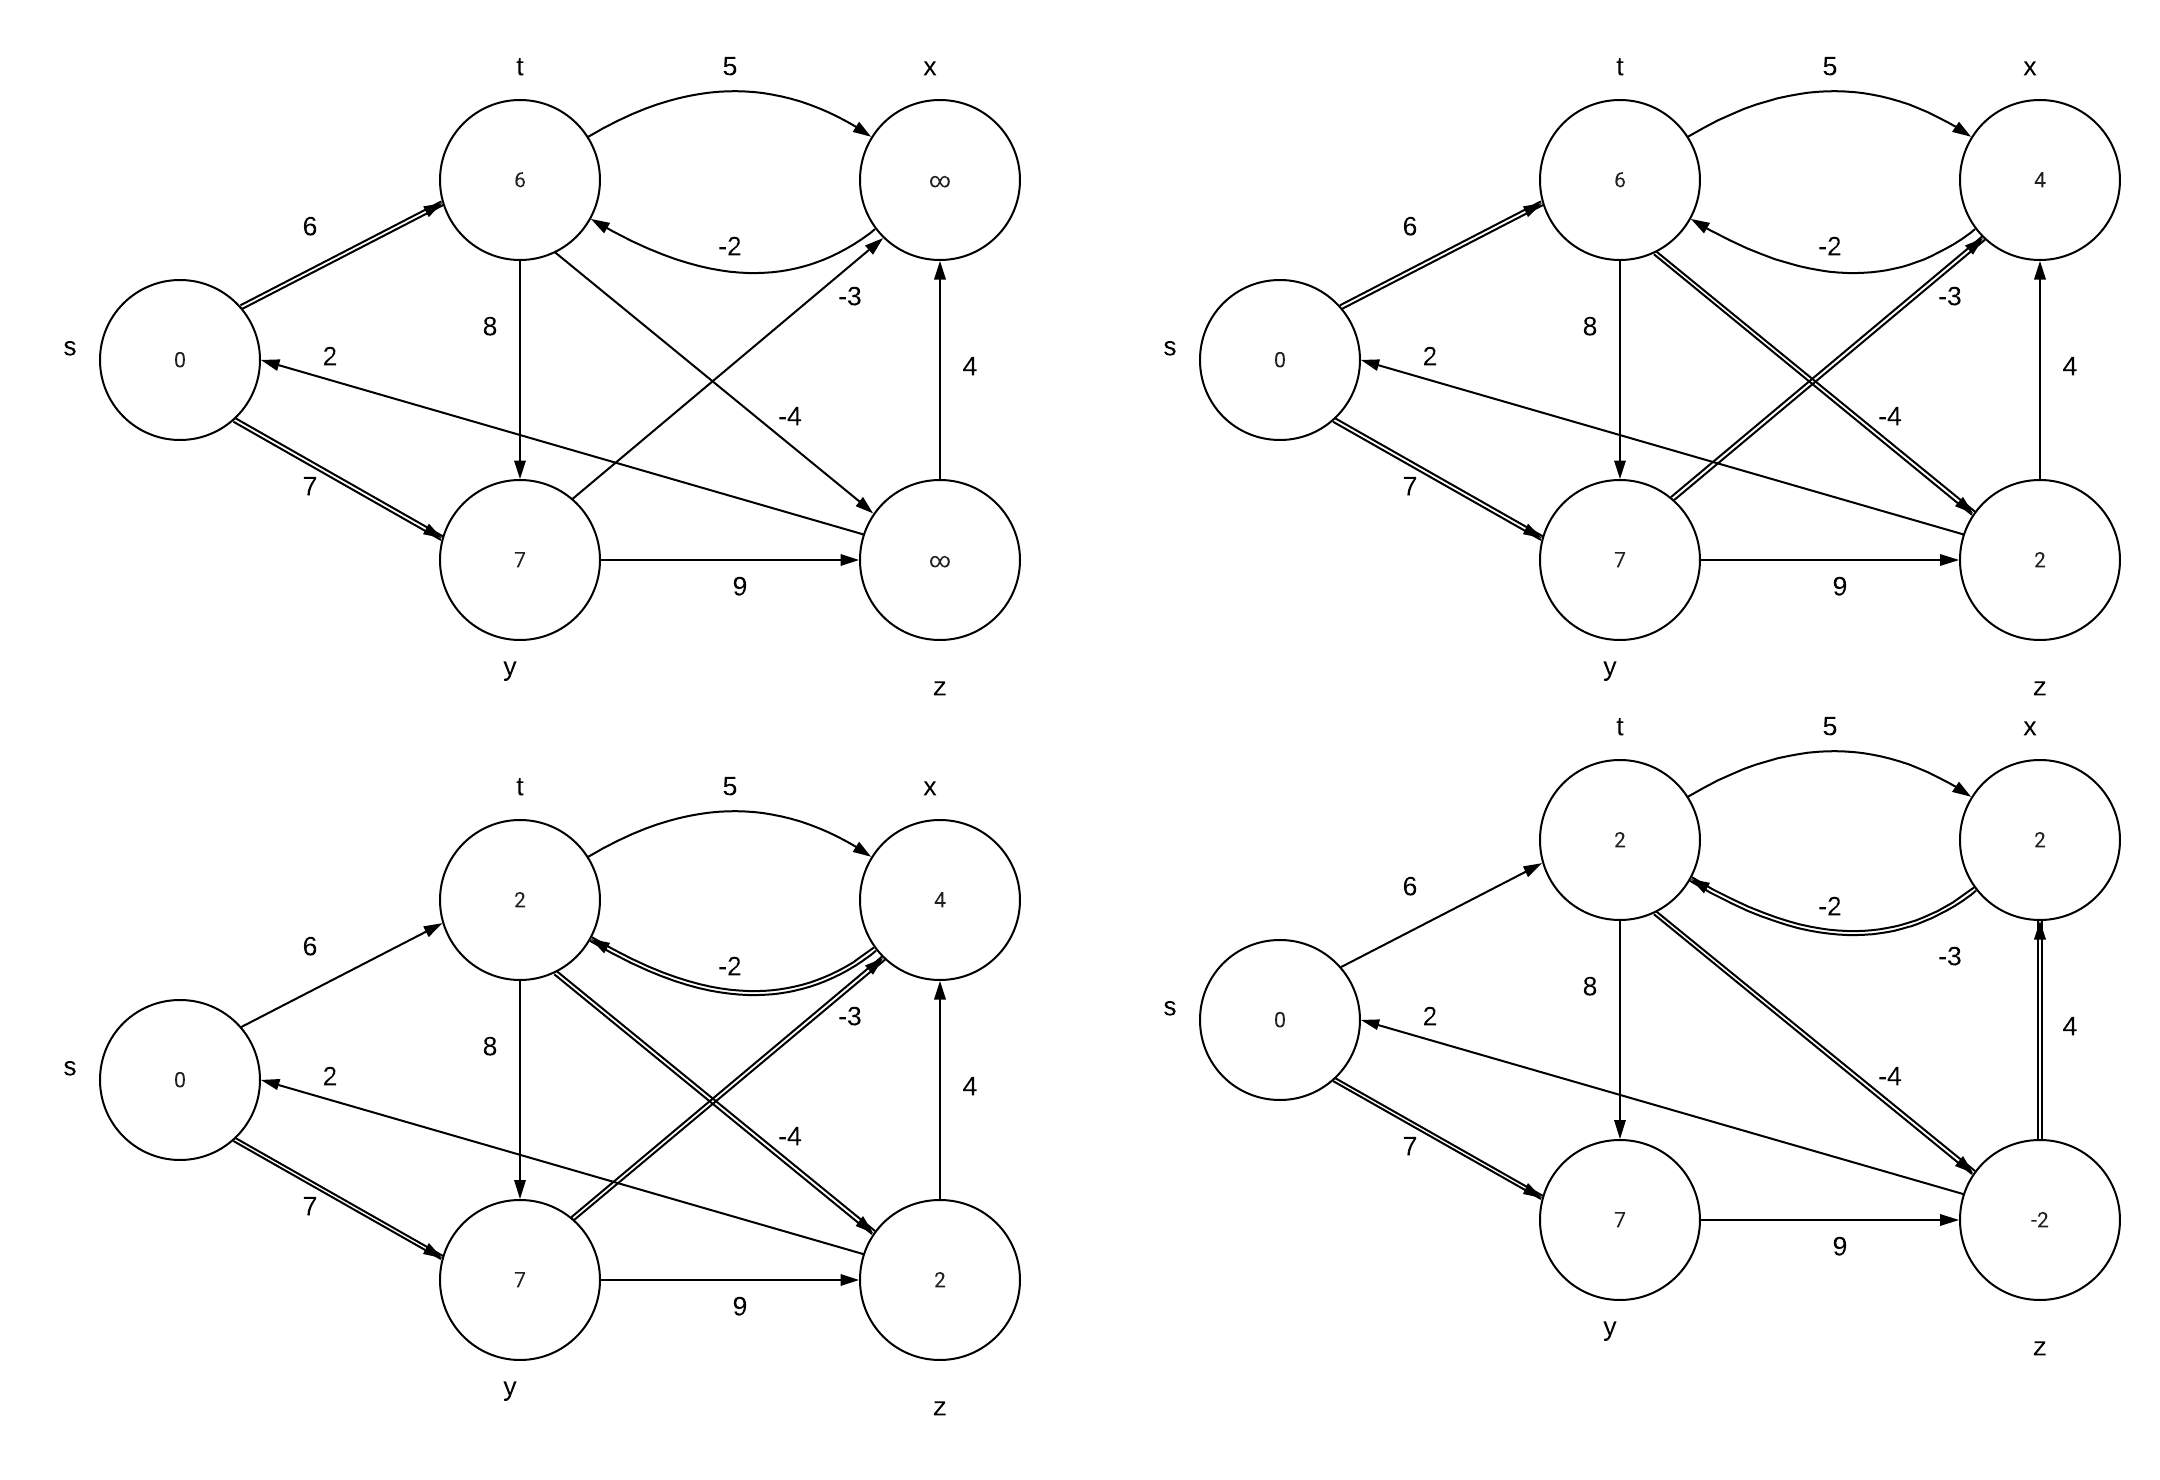
\includegraphics[width=\paperwidth]{images/bfinal.png}}
\end{center}

\end{document}
